%%%%%%%%%%%%%%%%%%%%%%%%%%%%%%%%%%%%% 
%% LE2I beamer template
%% Guillaume Lemaitre, October 2014
%%%%%%%%%%%%%%%%%%%%%%%%%%%%%%%%%%%%% 

\documentclass{beamer}

\usepackage[utf8]{inputenc}
\usepackage[T1]{fontenc} 
\usetheme{le2i} 

%% The amssymb package provides various useful mathematical symbols
\usepackage{amssymb}
%% The amsthm package provides extended theorem environments
\usepackage{amsthm}
%% amsmath for math environment
\usepackage{amsmath}

\DeclareMathOperator*{\argmin}{arg\,min}
\DeclareMathOperator*{\argmax}{arg\,max}
\DeclareMathOperator*{\sign}{sign}

%% Text packages
\usepackage[nolist]{acronym}
\usepackage{scalefnt}

%% figure package
\usepackage{standalone}
\usepackage{epsf,graphicx}
\usepackage{epstopdf}
\usepackage{subfigure}
\usepackage{transparent}

%% In order to draw some graphs
\usepackage{tikz,xifthen}
\usepackage{tikz-qtree}
\usepackage{adjustbox}
\usetikzlibrary{decorations.pathmorphing}
\usetikzlibrary{fit}
\usetikzlibrary{backgrounds}
\usetikzlibrary{shapes,arrows,shadows}
\usetikzlibrary{calc,decorations.pathreplacing,decorations.markings,positioning}
\usetikzlibrary{snakes,decorations.text,shapes,patterns}
% \usepackage{scalefnt,lmodern,booktabs}

%% Package for cross and tick symbols
\usepackage{pifont}
\newcommand{\tick}{\color{green!60!black!80}\ding{51}}
\newcommand{\cross}{\color{red!60!black!80}\ding{55}}
  % define the extra symbols
  \newcommand{\cmarkgLarge}{\text{\large \color{green!60!black!80}\ding{51}}}
  \newcommand{\cmarkrLarge}{\text{\large \color{red!60!black!80}\ding{51}}}
  \newcommand{\xmarkLarge}{\text{\large \color{red!60!black!80}\ding{55}}}
  \newcommand{\cmark}{\text{\color{green!60!black!80}\ding{51}}}
  \newcommand{\xmark}{\text{\color{red!60!black!80}\ding{55}}}

\setbeamercovered{transparent}
\resetcounteronoverlays{subfigure}

\usepackage{multirow}
\usepackage{biblatex}
\addbibresource{bibtex.bib}

\title{\Large{An optimization approach to segment breast lesions in ultra-sound images using clinically validated visual cues}}
\author{\scriptsize{Joan Massich\\ \texttt{joan.massich@u-bourgogne.fr}}}
\date{\scriptsize{Doctoral Day\\ 7\textsuperscript{th} October 2015}}

\institute{Universit\'e de Bourgogne} 

\newenvironment<>{redblock}[1]{%
  \begin{actionenv}#2%
    \def\insertblocktitle{#1}%
    \par%
    \mode<presentation>{%
      \setbeamercolor{block title}{fg=nicewhite,bg=red!75!black}
      \setbeamercolor{block body}{fg=niceblack,bg=red!20}
    }%
    \usebeamertemplate{block begin}}
  {\par\usebeamertemplate{block end}\end{actionenv}}

\newenvironment<>{greenblock}[1]{%
  \begin{actionenv}#2%
    \def\insertblocktitle{#1}%
    \par%
    \mode<presentation>{%
      \setbeamercolor{block title}{fg=nicewhite,bg=green!40!black}
      \setbeamercolor{block body}{fg=niceblack,bg=green!20}
    }%
    \usebeamertemplate{block begin}}
  {\par\usebeamertemplate{block end}\end{actionenv}}

%% Uncomment if you want to avoid thousand of bullet inside the menu
% \usepackage{etoolbox}
% \makeatletter
% \patchcmd{\slideentry}{\advance\beamer@xpos by1\relax}{}{}{}
% \def\beamer@subsectionentry#1#2#3#4#5{\advance\beamer@xpos by1\relax}%
% \makeatother

\begin{document}

\graphicspath{{images/generalFigures/}}

% Show the title page
\begin{frame}
  \titlepage
\end{frame}

% % Show the table of contents
% \begin{frame}
%   \tableofcontents[sectionstyle=show,subsectionstyle=show,subsubsectionstyle=hide]
% \end{frame}

\graphicspath{{images/generalFigures/}, {images/word_cloud/}}

\begin{frame}[plain]{}
  \begin{beamercolorbox}[wd=\paperwidth,ht=\paperheight]{frametitle}
    \begin{tikzpicture}
      \fill[azulunam, opacity=1] (0, 0) rectangle(100, 100);
      \node [anchor=center] (cloud) at 
        (0.5\paperwidth, 0.5\paperheight)
        {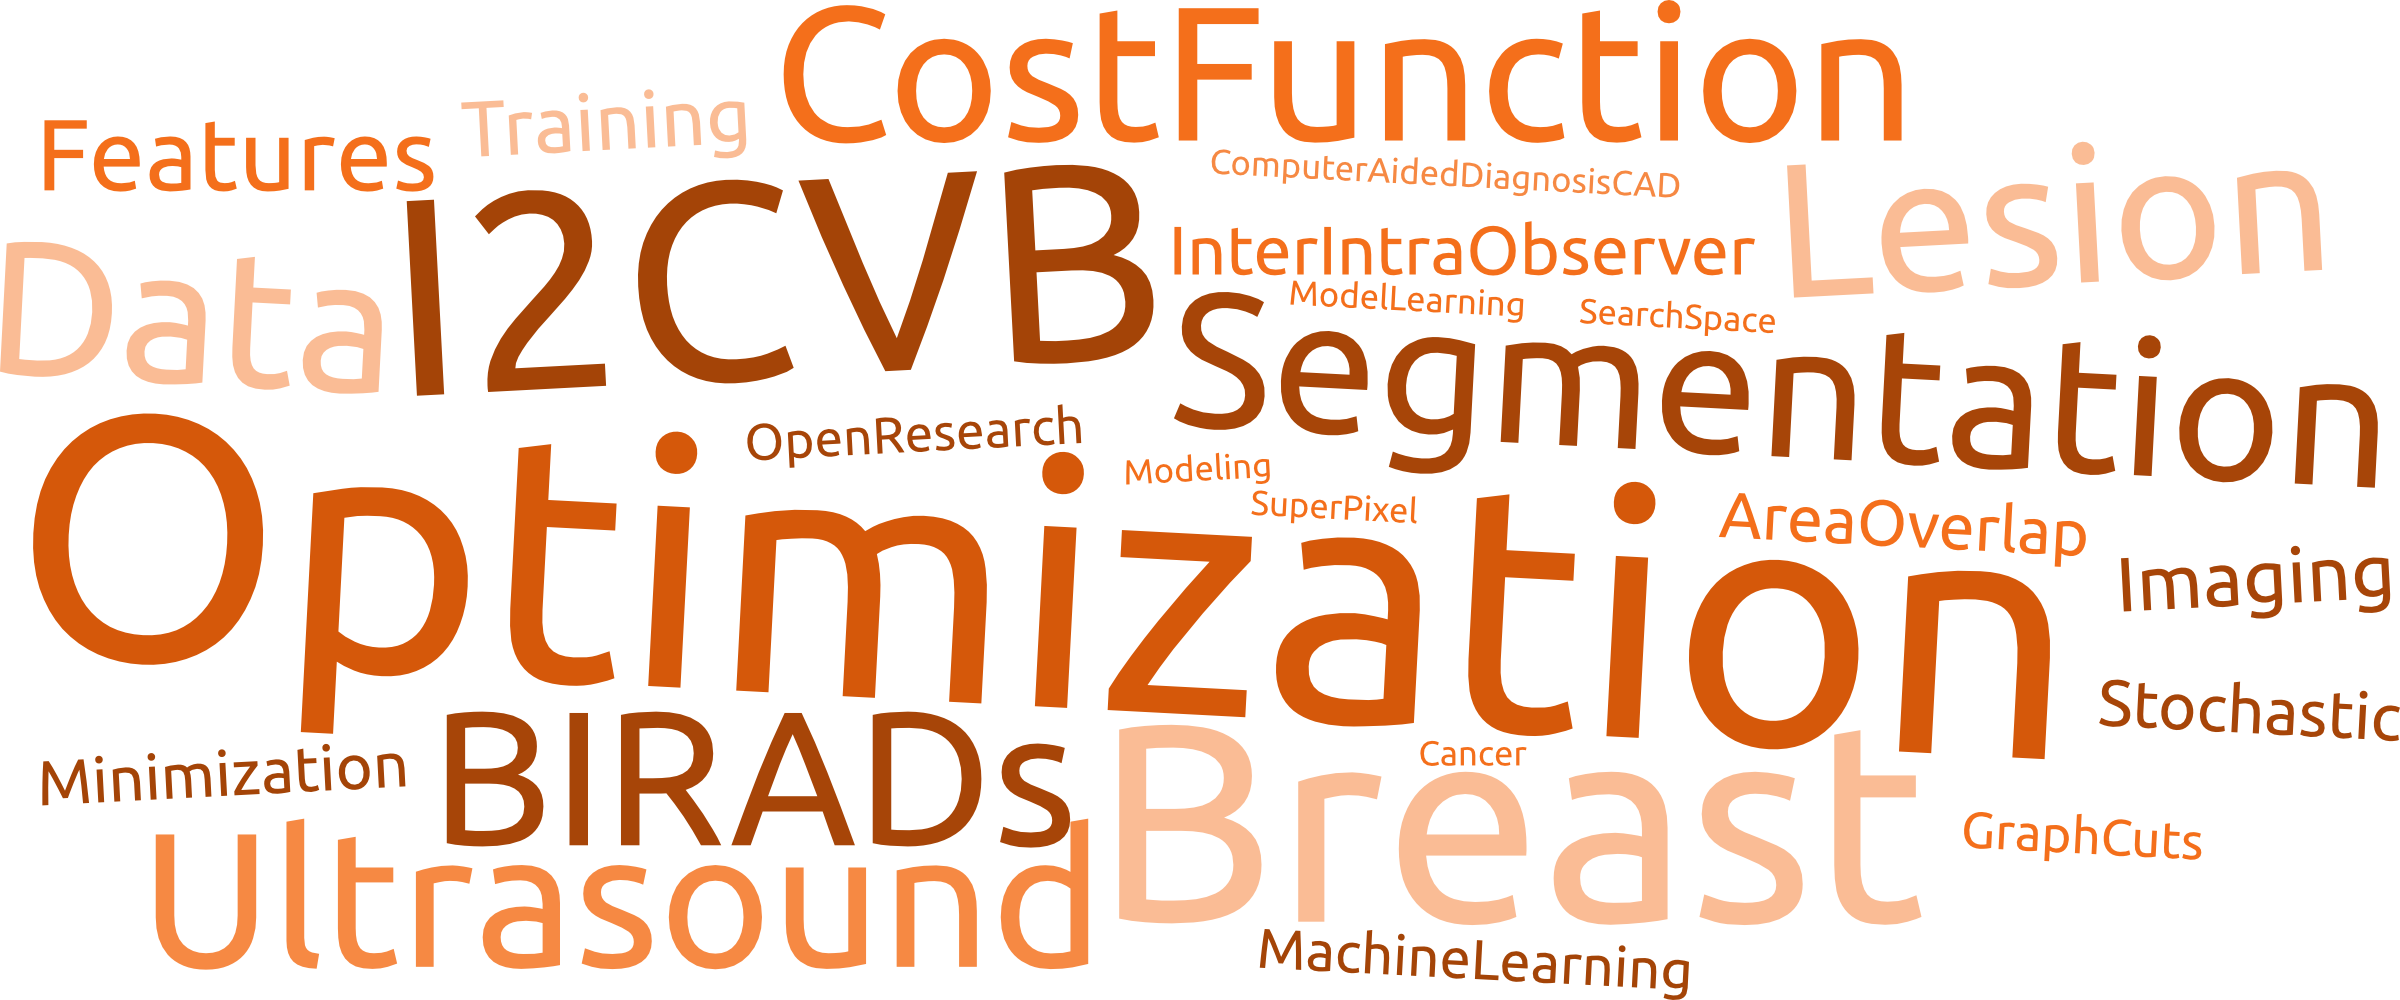
\includegraphics[width=.95\paperwidth]{orange_mix.png}};
    \end{tikzpicture}
  \end{beamercolorbox}
  % 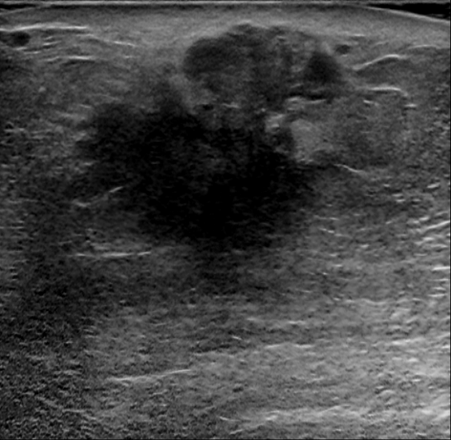
\includegraphics[trim=0 6 0 0,clip,height=.65\textheight]{a110105_094.png}~
\end{frame}


\begin{frame}[plain]{}
  \begin{beamercolorbox}[wd=\paperwidth,ht=\paperheight]{frametitle}
    \begin{tikzpicture}
      \fill[azulunam, opacity=1] (0, 0) rectangle(100, 100);
      \node [anchor=center] (cloud) at 
        (0.5\paperwidth, 0.5\paperheight)
        {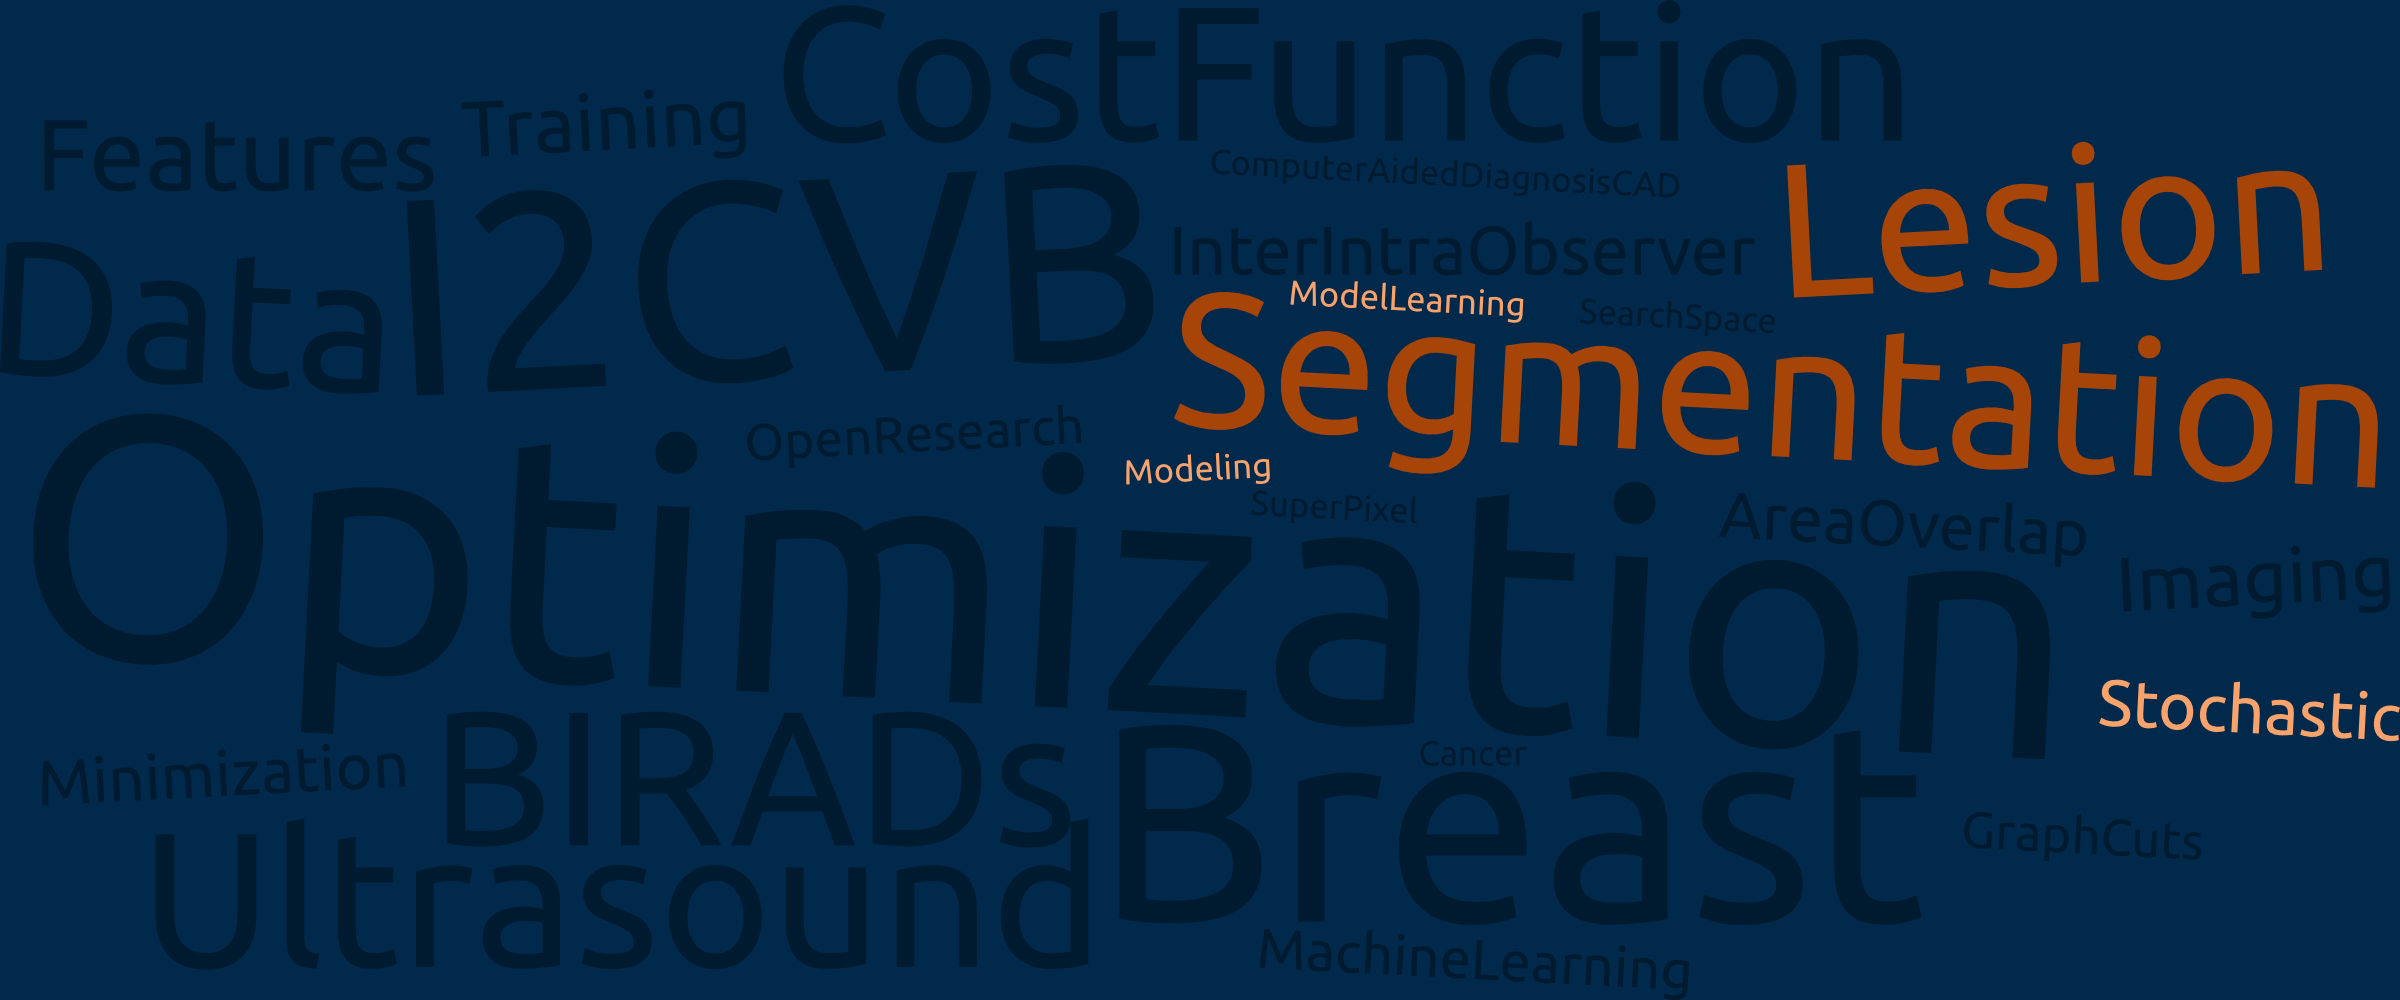
\includegraphics[width=.95\paperwidth]{highlight_prelude.png}};
    \end{tikzpicture}
  \end{beamercolorbox}
  % 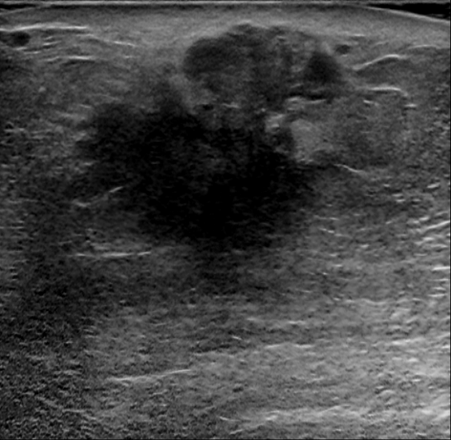
\includegraphics[trim=0 6 0 0,clip,height=.65\textheight]{a110105_094.png}~
\end{frame}

\begin{frame}[plain]\frametitle{Breast Lesion Segmentation in US images}
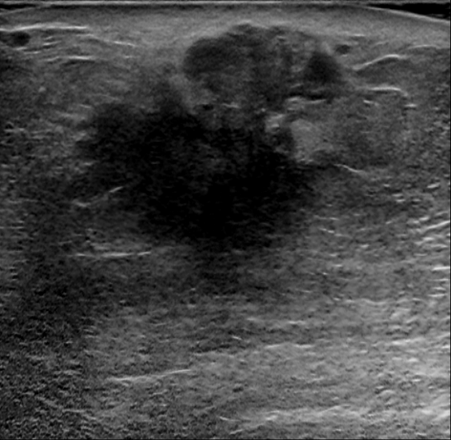
\includegraphics[trim=0 6 0 0,clip,height=.40\paperwidth]{a110105_094.png}~
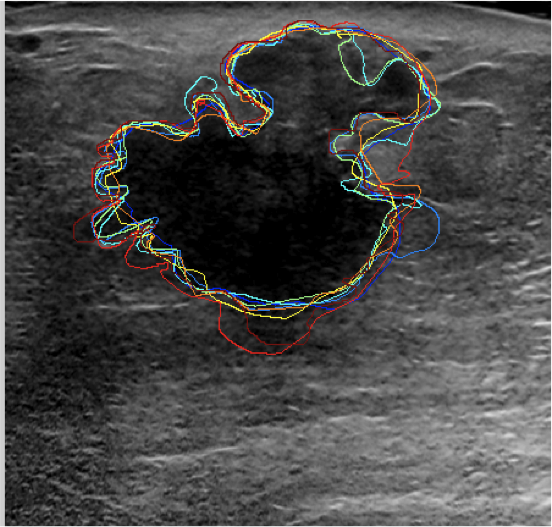
\includegraphics[trim=6 0 0 0,clip,height=.40\paperwidth]{segment.png}
\end{frame}



\begin{frame}
  \begin{beamercolorbox}[wd=\paperwidth,ht=\paperheight]{frametitle}
    \begin{tikzpicture}
      \fill[nicewhite, opacity=1] (0, 0) rectangle(1, 1);
      \node [anchor=center] (cloud) at 
        (0.5\paperwidth, 0.5\paperheight)
        {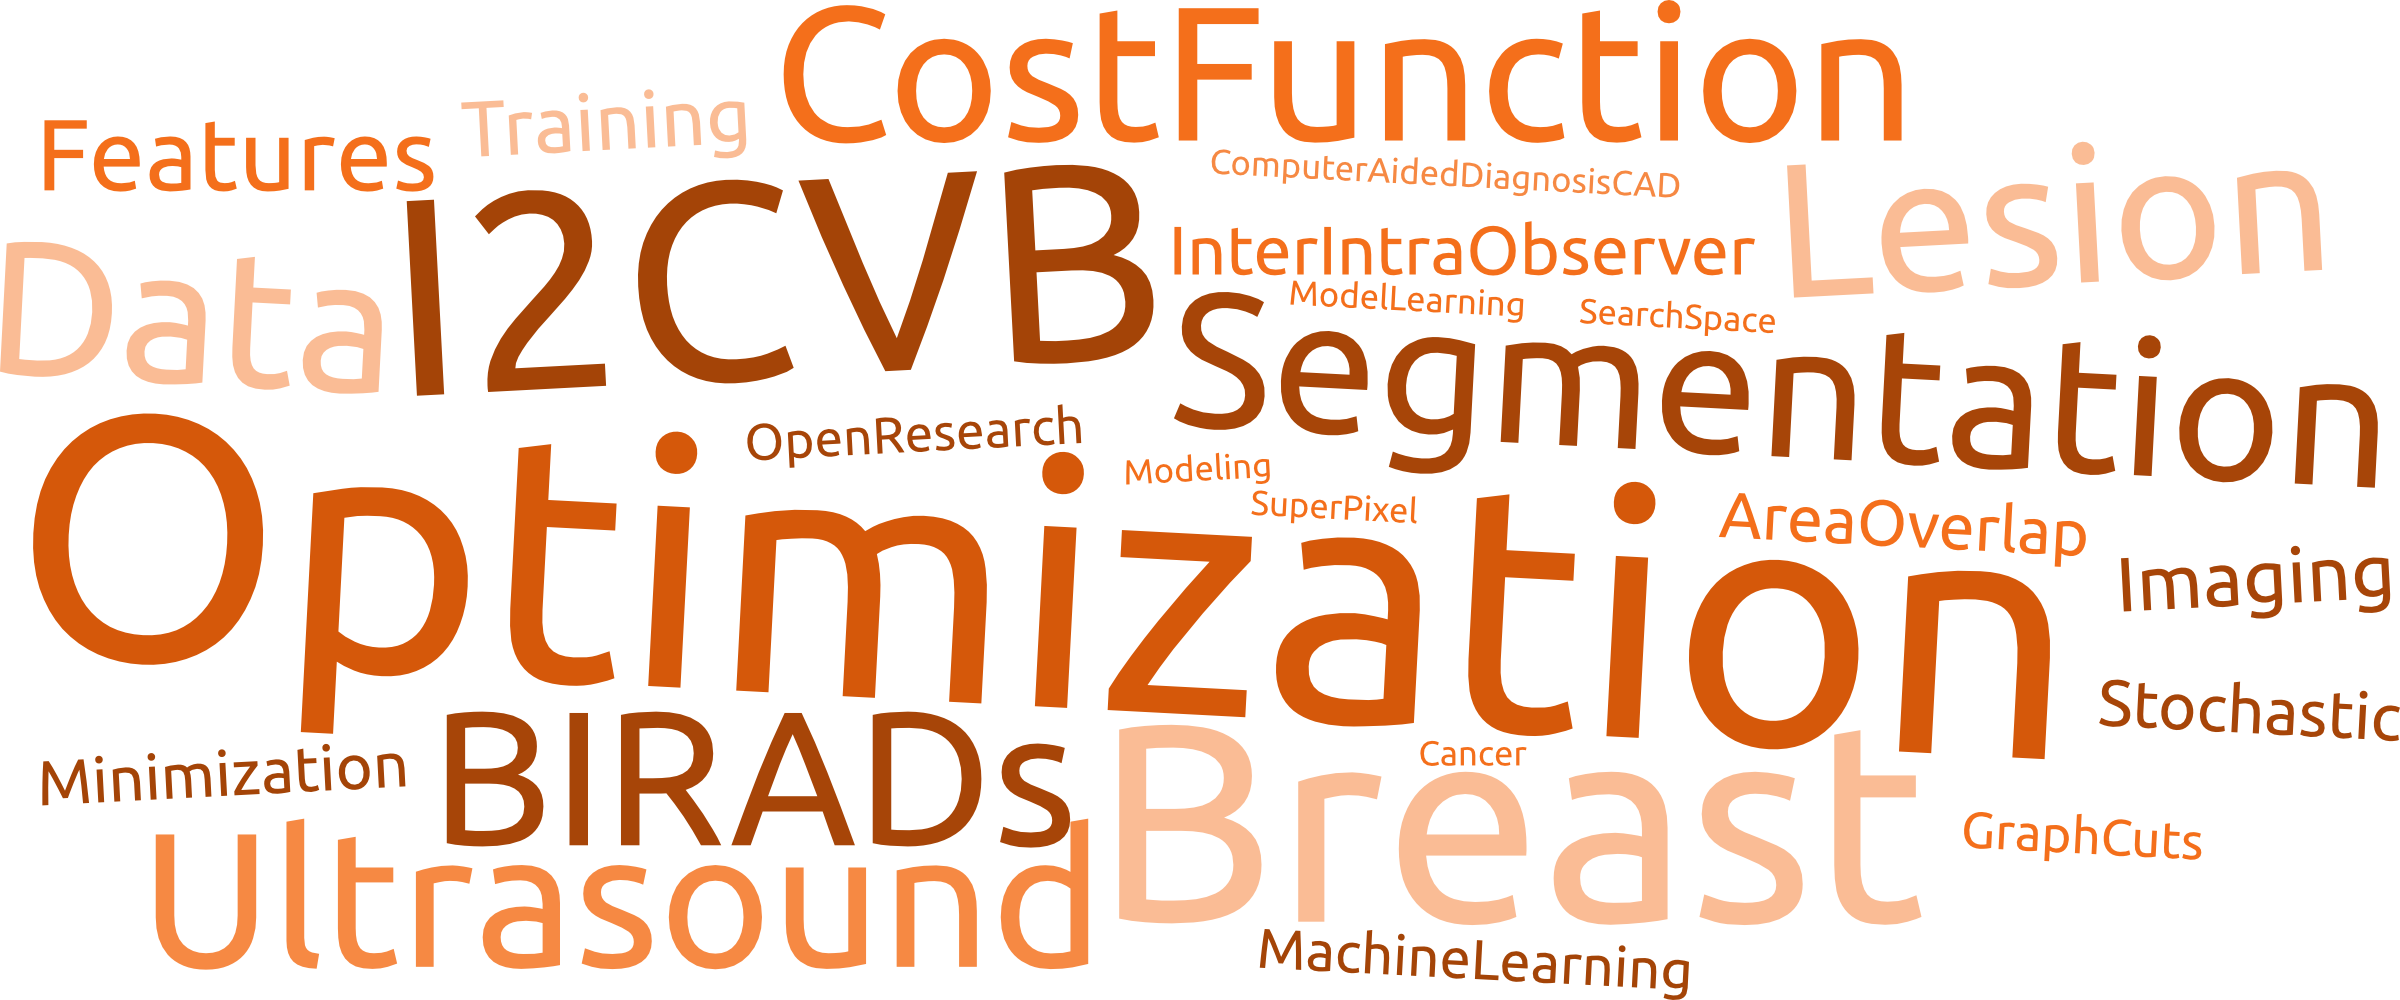
\includegraphics[width=.95\paperwidth]{orange_mix.png}};
    \end{tikzpicture}
  \end{beamercolorbox}
\end{frame}


\begin{frame}
  \begin{beamercolorbox}[wd=\paperwidth,ht=\paperheight]{frametitle}
    \begin{tikzpicture}
      \fill[nicewhite, opacity=1] (0, 0) rectangle(1, 1);
      \node [anchor=center] (cloud) at 
        (0.5\paperwidth, 0.5\paperheight)
        {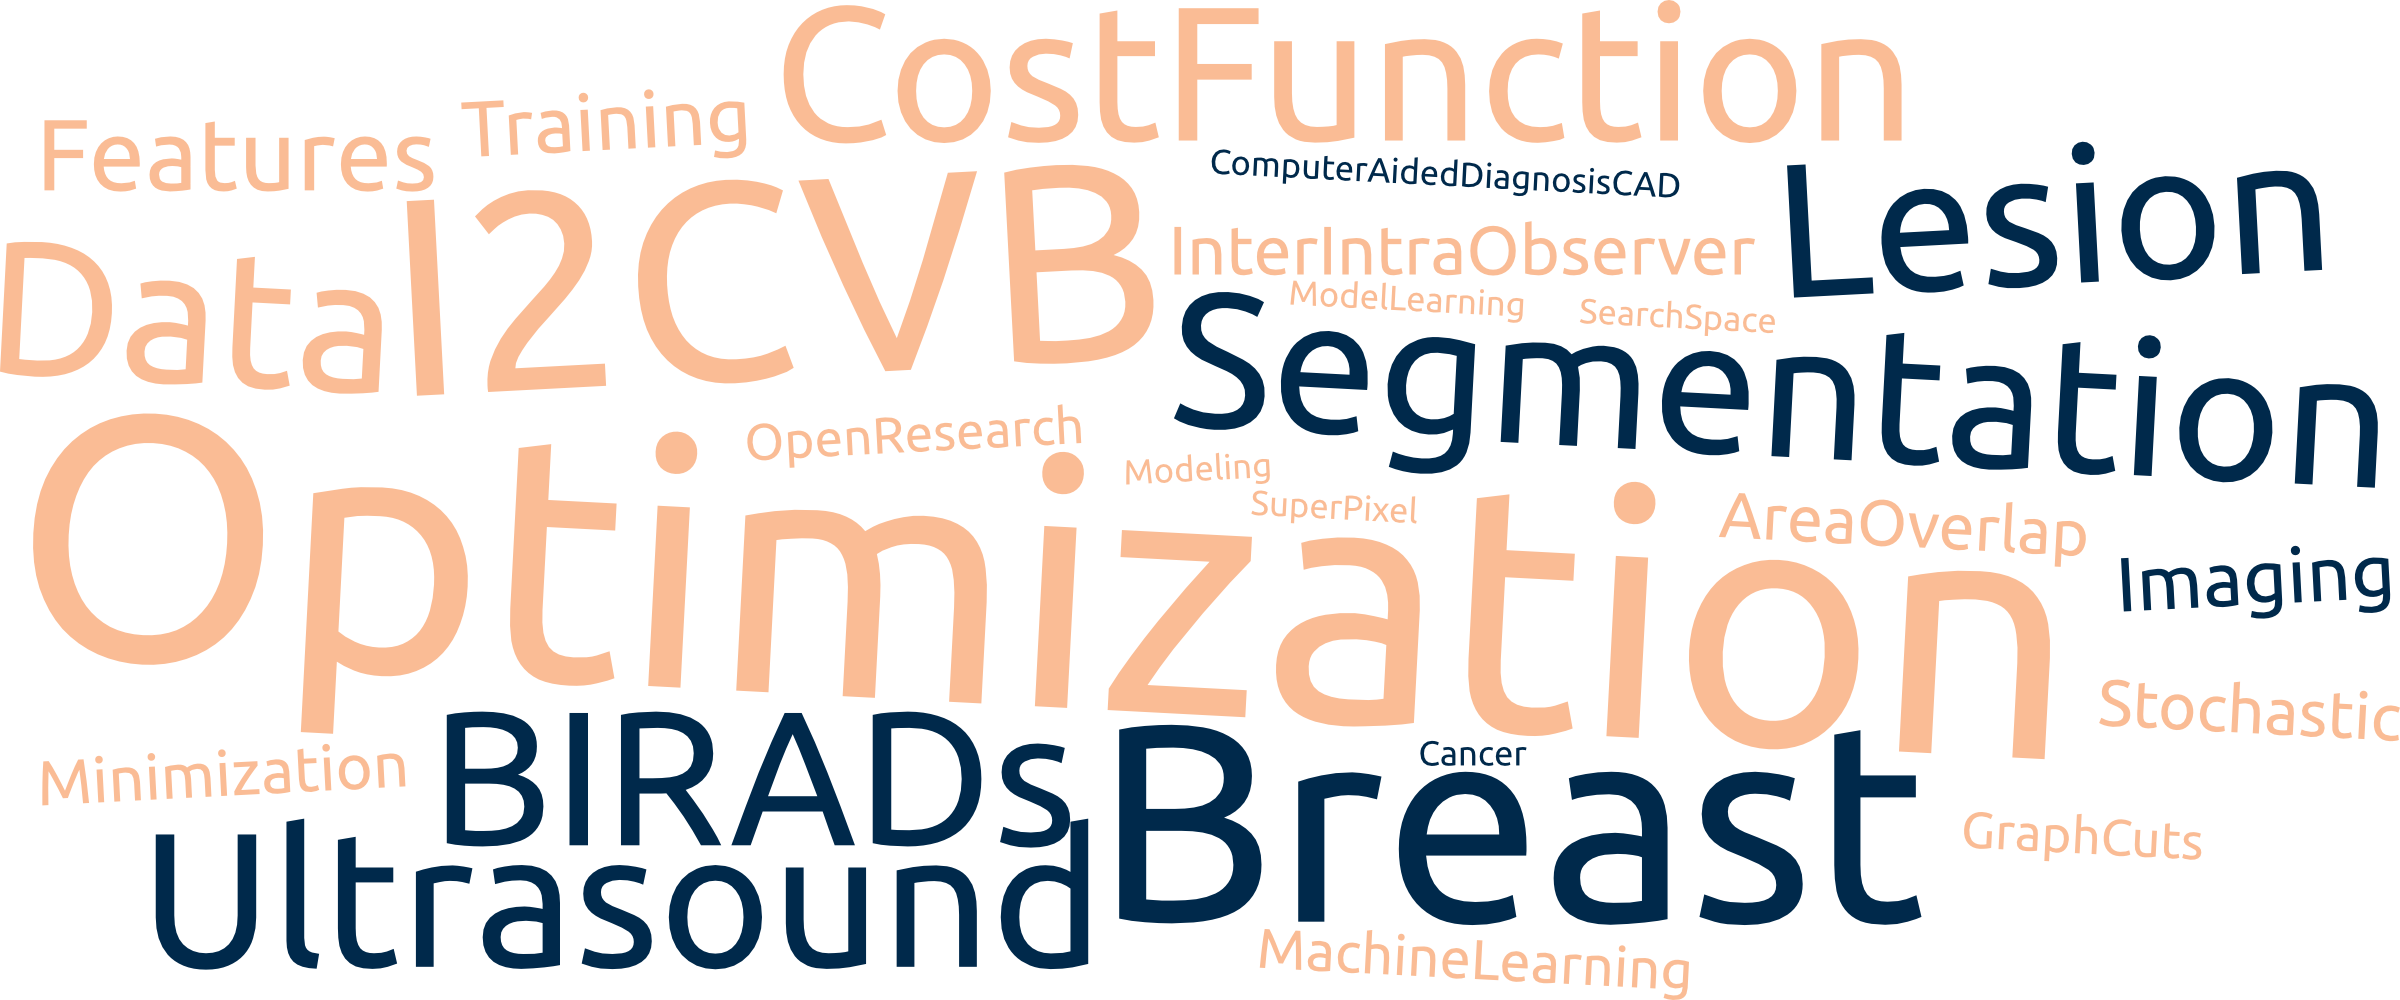
\includegraphics[width=.95\paperwidth]{intro.png}};
    \end{tikzpicture}
  \end{beamercolorbox}
\end{frame}


\begin{frame}
  \begin{beamercolorbox}[wd=\paperwidth,ht=\paperheight]{frametitle}
    \begin{tikzpicture}
      \fill[nicewhite, opacity=1] (0, 0) rectangle(1, 1);
      \node [anchor=center] (cloud) at 
        (0.5\paperwidth, 0.5\paperheight)
        {\includegraphics[width=.95\paperwidth]{method.png}};
    \end{tikzpicture}
  \end{beamercolorbox}
\end{frame}

\begin{frame}
  \begin{beamercolorbox}[wd=\paperwidth,ht=\paperheight]{frametitle}
    \begin{tikzpicture}
      \fill[nicewhite, opacity=1] (0, 0) rectangle(1, 1);
      \node [anchor=center] (cloud) at 
        (0.5\paperwidth, 0.5\paperheight)
        {\includegraphics[width=.95\paperwidth]{results.png}};
    \end{tikzpicture}
  \end{beamercolorbox}
\end{frame}

\section{Introduction}
\graphicspath{{chapters/introduction/figures/}}


\subsection{Motivations}

\begin{frame}{Motivations}
  % \frametitle{Introduction}
  % \framesubtitle{Motivations}
  \begin{block}{\small Statistics}
    \begin{figure}%
      \centering
      \hspace*{\fill}%
      \subfigure[][\tiny \# of cancer cases]{%
        \label{fig:stat1a}%
          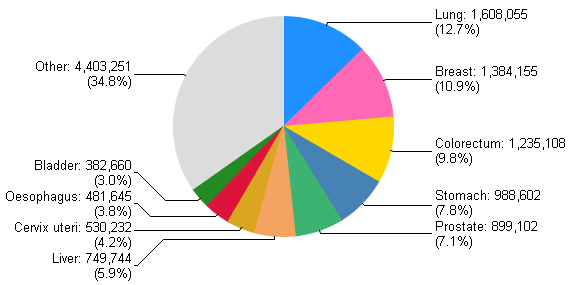
\includegraphics[width=.45\textwidth]{./images/statistics/repartitionCancerIncidence.png}}%
      \hfill%
      \subfigure[][\tiny \# of cancer deaths]{%
        \label{fig:stat1b}%
          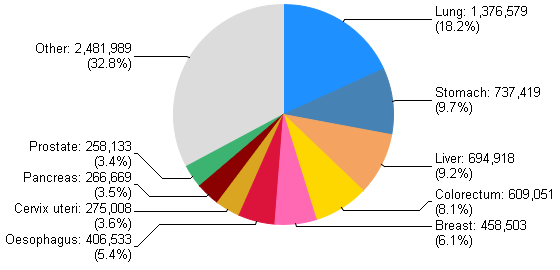
\includegraphics[width=.45\textwidth]{./images/statistics/repartitionCancerDeaths.png}}%
        \hspace*{\fill}%
      \label{fig:stat1}%
    \end{figure}
  \end{block}
  \begin{block}{\small Implications}\footnotesize
    \begin{itemize}
      \item 1.4 million cases per year
      \item 10.9\% of diagnosed cancers
      \item 5\textsuperscript{th} cause of cancer death (1\textsuperscript{th} females)
    \end{itemize}
  \end{block}
\end{frame}

\subsection{Screening}

\begin{frame}{Breast Imaging}
  % \frametitle{Introduction}
  % \framesubtitle{Screening}
  \begin{block}{\small Ultra-Sound(US) imaging, the most common adjunct modality}\footnotesize
    \begin{itemize}
    \item Ability to discern solid lesions typologies
    \item Lesions shielded by dense breast in Digital Mammography(DM) are distinguishable in US
    \end{itemize}
  \end{block}

  \begin{figure}%
     \centering
     \hspace*{\fill}%
     \subfigure[][\tiny DM]{%
       \label{fig:shielda}%
     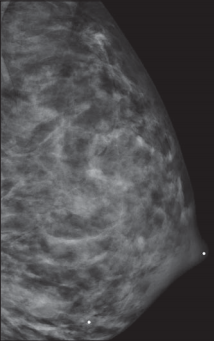
\includegraphics[trim = 0 0 0 20, clip,height=3.3cm]{mamo-us1.png}}
     \hfill%
     \subfigure[][\tiny DM, Region of Interest (ROI) ]{%
       \label{fig:shieldb}%
     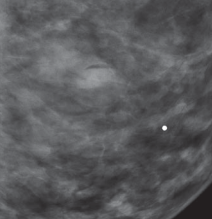
\includegraphics[trim = 0 0 0 20, clip,height=3.3cm]{mamo-us2.png}}
     \hfill%
     \subfigure[][\tiny Breast Ultra-Sound(BUS), ROI]{%
       \label{fig:shieldc}%
     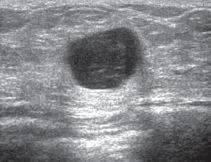
\includegraphics[trim = 10 20 10 0, clip,height=3.3cm]{mamo-us3.png}}
       \hspace*{\fill}%
    \label{fig:shield}%
  \end{figure}

\end{frame}

\subsection{Image formation, limitations and imaging perspectives}
\begin{frame}\frametitle{Breast structures under US screening}
\begin{columns}
\begin{column}{.48\textwidth}\vspace{-17pt}%\hspace{-1cm}
\begin{figure}\centering
\begin{tikzpicture}[scale=.5]
\begin{scriptsize}
	\tikzset{dot/.style={circle,draw=black,inner sep=0mm,minimum size=4pt}}
    \node[anchor=south west,inner sep=0] at (.2,.2) {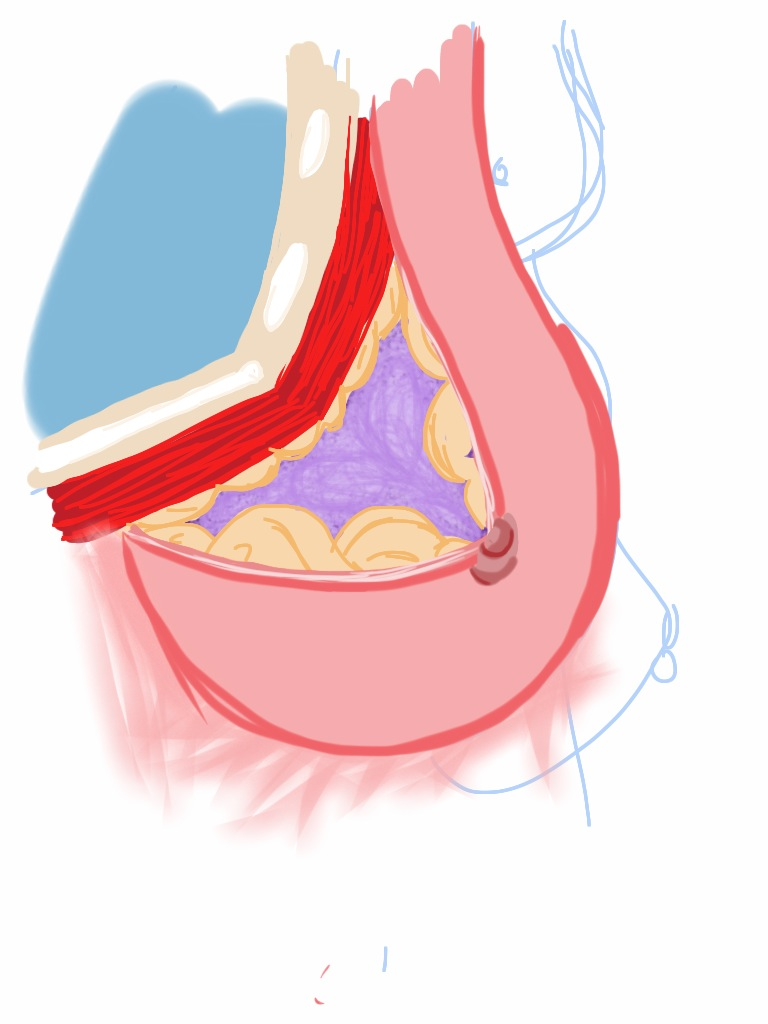
\includegraphics[trim = 20 190 80 20, clip,height=\textwidth]{pit.jpg}};
    \draw		(1.75,	7.75	) 	node[dot]	(AirCoord)			{}	
    				(2.5	,	5		) 	node[dot]	(PecCoord)			{}
    				(3.75,  7.75	) 	node[dot]	(CWCoord)			{}
    				(5,		5.40	) 	node[dot]	(TissueCoord)	{}
    				(2.5	,	3.65	) 	node[dot]	(SkinCoord)		{}
    				(3.75, 3.8	)  	node[dot]	(CooperCoord)	{}
    				(5.80, 5.40	)  	node[dot]	(FatCoord)			{};
 	   				
\draw	(AirCoord)	node[above left] (AirName) {Lungs (air)}
			node[below =of AirName.west, anchor=west] (PecName){Pectoral muscle}
   			(4.5,9.5)	node[anchor=west] (CWName){Chest-wall}
			node[below = of CWName,anchor=west,text width=2cm] (TissueName){Fibro-glandular tissue}
%    			(SkinCoord)
    			node[below= 1.8 of PecName.west, anchor=west ] (SkinName){Skin layers}
    			(CooperCoord |- SkinName)	node[text width=1.5cm,anchor= north west,inner sep=0mm,xshift=-5pt] (CooperName){Cooper's ligament}
    			(FatCoord) node[xshift=9,inner sep=0mm,anchor=west,text width=2cm] (FatName){Adipose tissue \emph{fat lobe}}
;   					 	
    \draw 	(PecCoord) -- (PecName)
    		   	(SkinCoord) -- (SkinName) 
				(CooperCoord) -- (CooperName)
%				(AirCoord) -- (AirName.south)
				(CWCoord) -- (CWName)
				(TissueCoord) -- (TissueName.west)
				(FatCoord) -- (FatName)
				;
%    
%    \draw[help lines,xstep=.5,ystep=.5] (0,0) grid (10,10);
%\foreach \x in {0,1,...,10} { \node [anchor=north] at (\x,0) {\x}; }
%\foreach \y in {0,1,...,10} { \node [anchor=east] at (0,\y) {\y}; });
\end{scriptsize}
\end{tikzpicture}
		\caption{Breast structure elements.}
		\end{figure}	
\end{column}

\begin{column}{.48\textwidth}
\begin{figure}
		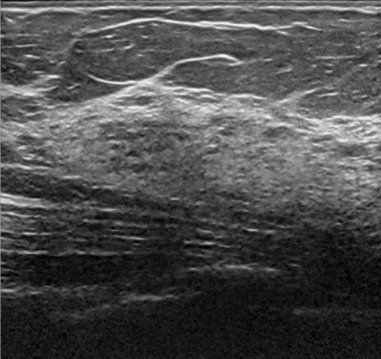
\includegraphics[height=.515\textheight]{sa1.png}
\caption{ Breast US image example.}
		\end{figure}	
\end{column}
\end{columns}
\end{frame}

\subsection{Image inspection to infer state of health}
%\subsection{Computer Aided Diagnosis (CAD)}

\begin{frame}\frametitle{State of health from image visual Inspection}
\setbeamercovered{transparent}
\begin{block}{Radiologic diagnosis error rates are similar to any other human visual inspection}
  \begin{itemize}
    \item Quality of the images.
    \item Ability to interpret the physical properties of the images.
  \end{itemize}
\end{block}
  \begin{enumerate}
    \item Double readings.
    \item Computer Aided Diagnosis(CAD).
  \end{enumerate}
\end{frame}


\definecolor{colorTheme}{RGB}{51,41,178}
\begin{frame}\frametitle{BI-RADs Lexicon}
  \framesubtitle{A standardized toolkit tested for diagnosis}
  \footnotesize
\begin{itemize}
\vspace{-5pt}
\item BKGD Echotexture :
			adipose, fibro-glandular, heterogeneous
\item Mass shape :
	\begin{tikzpicture}[baseline=(label.north)]
	\coordinate (rect) at (.5,.5);
	\coordinate (aux) at (.5,.53);

	\begin{tiny}
		\draw (0,0) rectangle (rect);
		\draw (0.25,0) node[minimum width=1cm,anchor=north](label){Oval};
		\draw [thick,colorTheme!80!white] (0.25,0.25) ellipse ( .2 and .08);
	\end{tiny}
	
	\begin{pgfonlayer}{background}
	\fill [green!30,rounded corners=2pt] ($ (label.west) !.65! (label.south west) $) rectangle (aux -| label.east);
	\end{pgfonlayer}
	\end{tikzpicture}
		\begin{tikzpicture}[baseline=(label.north)]
	\coordinate (rect) at (.5,.5);
	\coordinate (aux) at (.5,.53);

	\begin{tiny}
		\draw (0,0) rectangle (rect);
		\draw (0.25,0) node[minimum width=1cm,anchor=north](label){Round};
%				   (.25,.25) circle[fill,radius=.18,fill=red];
		\draw [thick,colorTheme!80!white]   (.25,.25) circle[radius=.18];
	\end{tiny}
	
	\begin{pgfonlayer}{background}
	\fill [red!30,rounded corners=2pt] ($ (label.west) !.65! (label.south west) $) rectangle (aux -| label.east);
	\end{pgfonlayer}
	\end{tikzpicture} 
		\begin{tikzpicture}[baseline=(label.north)]
	\coordinate (rect) at (.5,.5);
	\coordinate (aux) at (.5,.53);

	\begin{tiny}
		\draw (0,0) rectangle (rect);
		\draw (0.25,0) node[minimum width=1cm,anchor=north](label){Irregular};
		\draw [thick,colorTheme!80!white,rounded corners=2pt]   (.05,.25) -- (.1, .1)  -- (.2,.3) -- (.3,.2)  -- (.2,.05) -- (.35,.06) -- (.45,.25) -- (.4,.46) -- (.15,.3) -- (.1,.45) -- cycle;		
	\end{tiny}
	
	\begin{pgfonlayer}{background}
	\fill [red!30,rounded corners=2pt] ($ (label.west) !.65! (label.south west) $) rectangle (aux -| label.east);
	\end{pgfonlayer}
	\end{tikzpicture}
		\begin{tikzpicture}[baseline=(label.north)]
	\coordinate (rect) at (.5,.5);
	\coordinate (aux) at (.5,.53);

	\begin{tiny}
		\draw (0,0) rectangle (rect);
		\draw (0.25,0) node[minimum width=1cm,anchor=north](label){Lobular};
		\draw [thick,colorTheme!80!white,rounded corners=2pt]   (.05,.25) -- (.18,.15) -- (.25,.25) -- (.35,.15) -- (.45,.25) -- (.35,.35) -- (.25,.25) -- (.18,.35) -- cycle;
	\end{tiny}
	
	\begin{pgfonlayer}{background}
	\fill [orange!30,rounded corners=2pt] ($ (label.west) !.65! (label.south west) $) rectangle (aux -| label.east);
	\end{pgfonlayer}
	\end{tikzpicture}
\item Mass orientation :
		\begin{tikzpicture}[baseline=(label.north)]
	\coordinate (rect) at (.5,.5);
	\coordinate (aux) at (.5,.53);

	\begin{tiny}
		\draw (0,0) rectangle (rect);
		\draw (0.25,0) node[minimum width=1cm,anchor=north](label){Parallel};
		\draw[gray] (0,.44) -- (.5,.44);
		\draw[gray] (0,.47) -- (.5,.47);
		\draw [thick,colorTheme!80!white] (0.25,0.25) ellipse ( .15 and .06);
	\end{tiny}
	
	\begin{pgfonlayer}{background}
	\fill [green!30,rounded corners=2pt] ($ (label.west) !.65! (label.south west) $) rectangle (aux -| label.east);
	\end{pgfonlayer}
	\end{tikzpicture}
		\begin{tikzpicture}[baseline=(label.north)]
	\coordinate (rect) at (.5,.5);
	\coordinate (aux) at (.5,.53);

	\begin{tiny}
		\draw (0,0) rectangle (rect);
		\draw (0.25,0) node[anchor=north](label){Non-parallel};
		\draw[gray] (0,.44) -- (.5,.44);
		\draw[gray] (0,.47) -- (.5,.47);
		\draw [thick,colorTheme!80!white] (0.25,0.25) ellipse ( .06 and .15);
	\end{tiny}
	
	\begin{pgfonlayer}{background}
	\fill [red!30,rounded corners=2pt] ($ (label.west) !.65! (label.south west) $) rectangle (aux -| label.east);
	\end{pgfonlayer}
	\end{tikzpicture}
\item Mass margin :
		\begin{tikzpicture}[baseline=(label.north)]
	\coordinate (rect) at (.5,.5);
	\coordinate (aux) at (.5,.53);

	\begin{tiny}
		%\draw (0,0) rectangle (rect);
		\node[inner sep=0pt,anchor=south west]  at (0,0) {
\includegraphics[height=.5cm]{birads/circumscribed}};
		\draw (0.25,0) node[minimum width=1cm,anchor=north](label){Circumscribed};
	\end{tiny}
	
	\begin{pgfonlayer}{background}
	\fill [green!30,rounded corners=2pt] ($ (label.west) !.65! (label.south west) $) rectangle (aux -| label.east);
	\end{pgfonlayer}
	\end{tikzpicture}
		\begin{tikzpicture}[baseline=(label.north)]
	\coordinate (rect) at (.5,.5);
	\coordinate (aux) at (.5,.53);

	\begin{tiny}
		\node[inner sep=0pt,anchor=south west]  at (0,0) {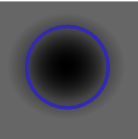
\includegraphics[height=.5cm]{birads/indistinct.png}};
		\draw (0.25,0) node[minimum width=1cm,anchor=north](label){Indistinct};
	\end{tiny}
	
	\begin{pgfonlayer}{background}
	\fill [red!30,rounded corners=2pt] ($ (label.west) !.65! (label.south west) $) rectangle (aux -| label.east);
	\end{pgfonlayer}
	\end{tikzpicture}
		\begin{tikzpicture}[baseline=(label.north)]
	\coordinate (rect) at (.5,.5);
	\coordinate (aux) at (.5,.53);

	\begin{tiny}
		\draw (0,0) rectangle (rect);
		\node[inner sep=0pt,anchor=south west]  at (.03,.12) {
\includegraphics[height=.3cm]{birads/angular}};
		\draw (0.25,0) node[minimum width=1cm,anchor=north](label){Angular};
	\end{tiny}
	
	\begin{pgfonlayer}{background}
	\fill [red!30,rounded corners=2pt] ($ (label.west) !.65! (label.south west) $) rectangle (aux -| label.east);
	\end{pgfonlayer}
	\end{tikzpicture}
		\begin{tikzpicture}[baseline=(label.north)]
	\coordinate (rect) at (.5,.5);
	\coordinate (aux) at (.5,.53);

	\begin{tiny}
			\draw (0,0) rectangle (rect);
		\node[inner sep=0pt,anchor=south west]  at (.05,.12) {
\includegraphics[height=.3cm]{birads/micro.pdf}};
		\draw (0.25,0) node[minimum width=1cm,anchor=north](label){Microlobulated};
	\end{tiny}
	
	\begin{pgfonlayer}{background}
	\fill [red!30,rounded corners=2pt] ($ (label.west) !.65! (label.south west) $) rectangle (aux -| label.east);
	\end{pgfonlayer}
	\end{tikzpicture}
		\begin{tikzpicture}[baseline=(label.north)]
	\coordinate (rect) at (.5,.5);
	\coordinate (aux) at (.5,.53);

	\begin{tiny}
		\draw (0,0) rectangle (rect);
		\node[inner sep=0pt,anchor=south west]  at (0.06,0.1) {
\includegraphics[height=.35cm]{birads/spiculated}};
		\draw (0.25,0) node[minimum width=1cm,anchor=north](label){Spiculated};
	\end{tiny}
	
	\begin{pgfonlayer}{background}
	\fill [red!30,rounded corners=2pt] ($ (label.west) !.65! (label.south west) $) rectangle (aux -| label.east);
	\end{pgfonlayer}
	\end{tikzpicture}
\item Lesion boundary :
		\begin{tikzpicture}[baseline=(label.north)]
	\coordinate (rect) at (.5,.5);
	\coordinate (aux) at (.5,.53);

	\begin{tiny}
%		\draw (0,0) rectangle (rect);
		\node[inner sep=0pt,anchor=south west]  at (0,0) {
\includegraphics[height=.5cm]{birads/Abrupt}};
		\draw (0.25,0) node[minimum width=1cm,anchor=north](label){Abrupt Interface};
	\end{tiny}
	
	\begin{pgfonlayer}{background}
	\fill [green!30,rounded corners=2pt] ($ (label.west) !.65! (label.south west) $) rectangle (aux -| label.east);
	\end{pgfonlayer}
	\end{tikzpicture}
		\begin{tikzpicture}[baseline=(label.north)]
	\coordinate (rect) at (.5,.5);
	\coordinate (aux) at (.5,.53);

	\begin{tiny}
%		\draw (0,0) rectangle (rect);
		\node[inner sep=0pt,anchor=south west]  at (0,0) {
\includegraphics[height=.5cm]{birads/halo}};
		\draw (0.25,0) node[minimum width=1cm,anchor=north](label){Echogenic halo};
	\end{tiny}
	
	\begin{pgfonlayer}{background}
	\fill [red!30,rounded corners=2pt] ($ (label.west) !.65! (label.south west) $) rectangle (aux -| label.east);
	\end{pgfonlayer}
	\end{tikzpicture}
\item Echo pattern :
		\begin{tikzpicture}[baseline=(label.north)]
	\coordinate (rect) at (.5,.5);
	\coordinate (aux) at (.5,.53);

	\begin{tiny}
		\node[inner sep=0pt,anchor=south west]  at (0,0) {
\includegraphics[height=.5cm]{birads/anechoic}};
		\draw (0.25,0) node[minimum width=1cm,anchor=north](label){Anechoic};
	\end{tiny}
	
	\begin{pgfonlayer}{background}
	\fill [green!30,rounded corners=2pt] ($ (label.west) !.65! (label.south west) $) rectangle (aux -| label.east);
	\end{pgfonlayer}
	\end{tikzpicture}
		\begin{tikzpicture}[baseline=(label.north)]
	\coordinate (rect) at (.5,.5);
	\coordinate (aux) at (.5,.53);

	\begin{tiny}
		\node[inner sep=0pt,anchor=south west]  at (0,0) {
\includegraphics[height=.5cm]{birads/hyperechoic}};
		\draw (0.25,0) node[minimum width=1cm,anchor=north](label){Hyperechoic};
	\end{tiny}
	
	\begin{pgfonlayer}{background}
	\fill [green!30,rounded corners=2pt] ($ (label.west) !.65! (label.south west) $) rectangle (aux -| label.east);
	\end{pgfonlayer}
	\end{tikzpicture}
		\begin{tikzpicture}[baseline=(label.north)]
	\coordinate (rect) at (.5,.5);
	\coordinate (aux) at (.5,.53);

	\begin{tiny}
\node[inner sep=0pt,anchor=south west]  at (0,0) {
\includegraphics[height=.5cm]{birads/complex.png}};
		\draw (0.25,0) node[minimum width=1cm,anchor=north](label){Complex};
	\end{tiny}
	
	\begin{pgfonlayer}{background}
	\fill [red!30,rounded corners=2pt] ($ (label.west) !.65! (label.south west) $) rectangle (aux -| label.east);
	\end{pgfonlayer}
	\end{tikzpicture}
		\begin{tikzpicture}[baseline=(label.north)]
	\coordinate (rect) at (.5,.5);
	\coordinate (aux) at (.5,.53);

	\begin{tiny}
%		\draw (0,0) rectangle (rect);
		\node[inner sep=0pt,anchor=south west]  at (0,0) {
\includegraphics[height=.5cm]{birads/isoechoic}};
		\draw (0.25,0) node[minimum width=1cm,anchor=north](label){Isoechoic};
	\end{tiny}
	
	\begin{pgfonlayer}{background}
	\fill [orange!30,rounded corners=2pt] ($ (label.west) !.65! (label.south west) $) rectangle (aux -| label.east);
	\end{pgfonlayer}
	\end{tikzpicture}
		\begin{tikzpicture}[baseline=(label.north)]
	\coordinate (rect) at (.5,.5);
	\coordinate (aux) at (.5,.53);

	\begin{tiny}
		\node[inner sep=0pt,anchor=south west]  at (0,0) {
\includegraphics[height=.5cm]{birads/hypoechoic}};
		\draw (0.25,0) node[minimum width=1cm,anchor=north](label){Hypoechoic};
	\end{tiny}
	
	\begin{pgfonlayer}{background}
	\fill [orange!30,rounded corners=2pt] ($ (label.west) !.65! (label.south west) $) rectangle (aux -| label.east);
	\end{pgfonlayer}
	\end{tikzpicture}
\item Posterior acoustic pattern : 
		\begin{tikzpicture}[baseline=(label.north)]
	\coordinate (rect) at (.5,.5);
	\coordinate (aux) at (.5,.53);

	\begin{tiny}
\node[inner sep=0pt,anchor=south west]  at (0,0) {
\includegraphics[height=.5cm]{birads/shadow}};
		\draw (0.25,0) node[minimum width=1cm,anchor=north](label){Shadowing};
	\end{tiny}
	
	\begin{pgfonlayer}{background}
	\fill [red!30,rounded corners=2pt] ($ (label.west) !.65! (label.south west) $) rectangle (aux -| label.east);
	\end{pgfonlayer}
	\end{tikzpicture}
		\begin{tikzpicture}[baseline=(label.north)]
	\coordinate (rect) at (.5,.5);
	\coordinate (aux) at (.5,.53);

	\begin{tiny}
\node[inner sep=0pt,anchor=south west]  at (0,0) {
\includegraphics[height=.5cm]{birads/combined}};
		\draw (0.25,0) node[minimum width=1cm,anchor=north](label){Combined};
	\end{tiny}
	
	\begin{pgfonlayer}{background}
	\fill [red!30,rounded corners=2pt] ($ (label.west) !.65! (label.south west) $) rectangle (aux -| label.east);
	\end{pgfonlayer}
	\end{tikzpicture}
		\begin{tikzpicture}[baseline=(label.north)]
	\coordinate (rect) at (.5,.5);
	\coordinate (aux) at (.5,.53);

	\begin{tiny}
\node[inner sep=0pt,anchor=south west]  at (0,0) {
\includegraphics[height=.5cm]{birads/enhance}};
		\draw (0.25,0) node[minimum width=1cm,anchor=north](label){Enhancement};
	\end{tiny}
	
	\begin{pgfonlayer}{background}
	\fill [orange!30,rounded corners=2pt] ($ (label.west) !.65! (label.south west) $) rectangle (aux -| label.east);
	\end{pgfonlayer}
	\end{tikzpicture}
		\begin{tikzpicture}[baseline=(label.north)]
	\coordinate (rect) at (.5,.5);
	\coordinate (aux) at (.5,.53);

	\begin{tiny}
\node[inner sep=0pt,anchor=south west]  at (0,0) {
\includegraphics[height=.5cm]{birads/hypoechoic}};
		\draw (0.25,0) node[minimum width=1cm,anchor=north](label){No pattern};
	\end{tiny}
	
	\begin{pgfonlayer}{background}
	\fill [orange!30,rounded corners=2pt] ($ (label.west) !.65! (label.south west) $) rectangle (aux -| label.east);
	\end{pgfonlayer}
	\end{tikzpicture}
\end{itemize}

\footnotetext{~\tikz[baseline=(x),inner sep=1.5pt] {\coordinate (x) at (0,-3pt); \node[fill=green!30,rounded corners=2pt,anchor=base,minimum size=10pt] {};} benign, \tikz[baseline=(x),inner sep=1.5pt] {\coordinate (x) at (0,-3pt); \node[fill=red!30,rounded corners=2pt,anchor=base,minimum size=10pt] {};} malignant and \tikz[baseline=(x),inner sep=1.5pt] {\coordinate (x) at (0,-3pt); \node[fill=orange!30,rounded corners=2pt,anchor=base,minimum size=10pt] {};} undetermined 
  \\
\vspace{2pt}}
\end{frame}

\begin{frame}\frametitle{Take away}
  \framesubtitle{Accurate delineations to develop CAD systems for BUS}
\begin{figure}
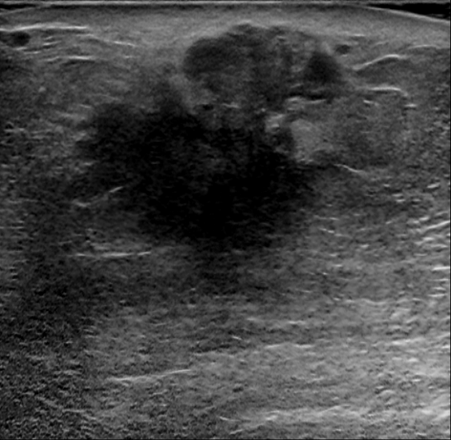
\includegraphics[trim=0 6 0 0,clip,height=.5\textheight]{a110105_094.png}~
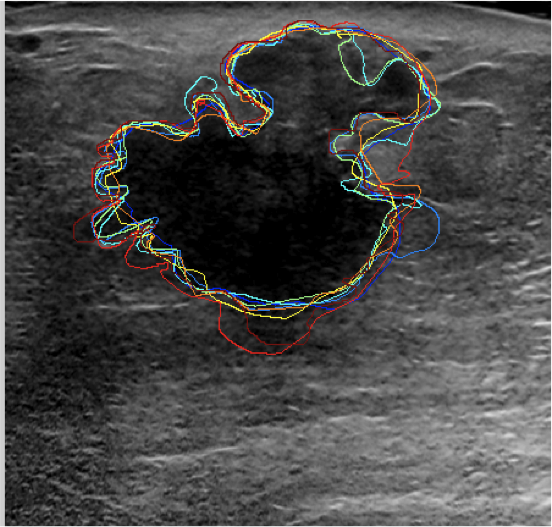
\includegraphics[trim=6 0 0 0,clip,height=.5\textheight]{segment.png}
\end{figure}
\end{frame}


\section{Optimization Based Segmentation}

\begin{frame}
  \begin{beamercolorbox}[wd=\paperwidth,ht=\paperheight]{frametitle}
    \begin{tikzpicture}
      \fill[nicewhite, opacity=1] (0, 0) rectangle(1, 1);
      \node [anchor=center] (cloud) at 
        (0.5\paperwidth, 0.5\paperheight)
        {\includegraphics[width=.95\paperwidth]{./images/word_cloud/method.png}};
    \end{tikzpicture}
  \end{beamercolorbox}
\end{frame}
\graphicspath{{chapters/method/figures/}}

\subsection{forumulation}
\begin{frame}\frametitle{Optimization}
\framesubtitle{For image segmentation}

\begin{equation*}
\hat{\omega} = \arg \min_{\substack{\omega}} \,U(\omega)
\end{equation*} 

\begin{block}{Considerations}
  \begin{itemize}
    \item Search Space $\mathcal{W}$
    \item Cost Function $U(\cdot)$
      \item Minimization Strategy
  \end{itemize}
\end{block}
\end{frame}

\begin{frame}\frametitle{Image Segmentation by Optimization}
\framesubtitle{The Metric Labeling Problem}

\vspace{-0.5cm}
\begin{equation*}
\hat{\omega} = \arg \min_{\substack{\omega}} \,U(\omega)
\end{equation*} 

\vspace{-0.2cm}
\begin{equation*}
U(\omega) = \sum_{s\in S} D_s(\omega_s) + \sum_{s}\sum_{r \in \mathcal{N}_{s}} V_{s,r}(\omega_s,\omega_r)
\end{equation*} 

% \vspace{-1cm}
\begin{columns}
\begin{column}{.4\textwidth}
  \begin{block}{Considerations}
    \begin{itemize}
        \item Image as a discrete set $\mathcal{S}$
        \item Search Space $\mathcal{W}$\\
          {\small($\omega_s = l$), $l \in \mathcal{L}$, $\forall s \in \mathcal{S}$}
        \item Cost Function
        \item Minimization Strategy
    \end{itemize}
  \end{block}
\end{column}
\begin{column}{.6\textwidth}
  \begin{block}{Cost function}
    \begin{itemize}
        \item $D_s$ is the Data-Term
        \item $D_s(\omega_s=l_\cmark) << D_s(\omega_s=l_\xmark)$
        \item $V_{s,r}$ is the Pairwise-Term
        \item \[ V_{s,r}(\omega_s,\omega_r) = 
              \begin{cases}
                \beta, & \text{if } \omega_s \ne \omega_r\\
                0,              & \text{otherwise}
              \end{cases} \]
    \end{itemize}
  \end{block}
\end{column}
\end{columns}
\end{frame}

\subsection{Interpretation}


\frame{\frametitle{The Metric Labeling Problem}%\framesubtitle{\insertsubsection}
  \framesubtitle{Interpretation of the Cost function terms}
	\begin{footnotesize}

  \begin{block}{$D_s(\omega_s = l)$ Interpretation}\tiny
    \begin{figure}%
      \centering
      \hspace*{\fill}%
        \subfigure[][\tiny $l$ is fat]{%
          \label{fig:dataTermb}%
        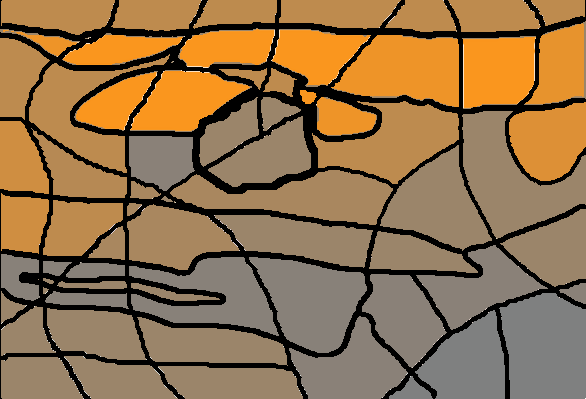
\includegraphics[height=1.9cm]{b.png}}
        \hfill%
        \subfigure[][\tiny $l$ is lungs]{%
          \label{fig:dataTermc}%
        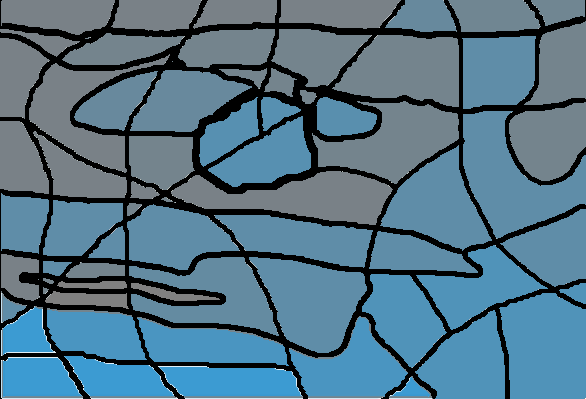
\includegraphics[height=1.9cm]{c.png}}
        \hspace*{\fill}%
          \subfigure[][\tiny $l$ is lesion]{%
            \label{fig:dataTermd}%
          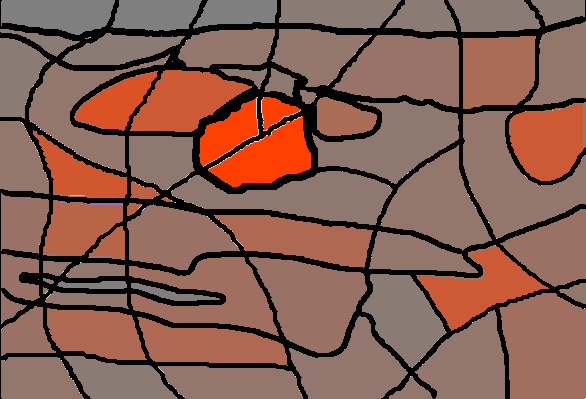
\includegraphics[height=1.9cm]{d.png}}
          \hspace*{\fill}%
            \label{fig:dataTerm}%
    \end{figure}
  \end{block}
	\vspace{-5pt}
  \begin{block}{$V_{s,r}(\omega_s,\omega_r)$ Interpretation}\tiny
  \begin{figure}%
     \centering
     \hspace*{\fill}%
     \subfigure[]{%
       \label{fig:smoothTermb}%
     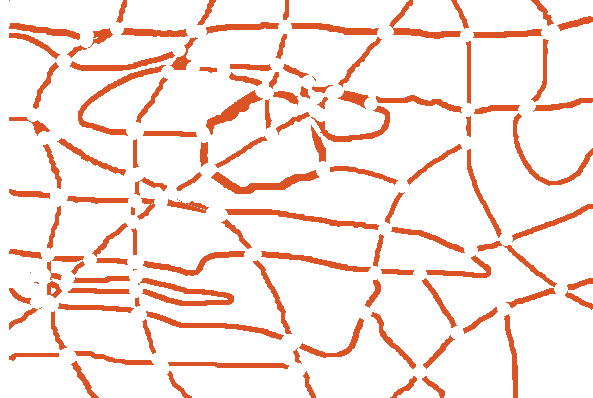
\includegraphics[height=1.9cm]{e.png}}
     \hfill%
     \subfigure[]{%
       \label{fig:smoothTermc}%
     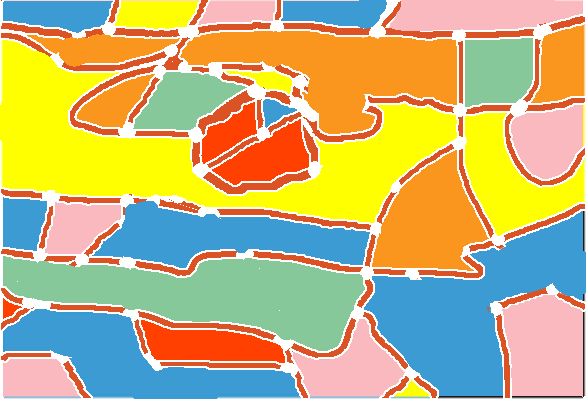
\includegraphics[height=1.9cm]{f.png}}
       \hspace*{\fill}%
     \subfigure[]{%
       \label{fig:smoothTermd}%
     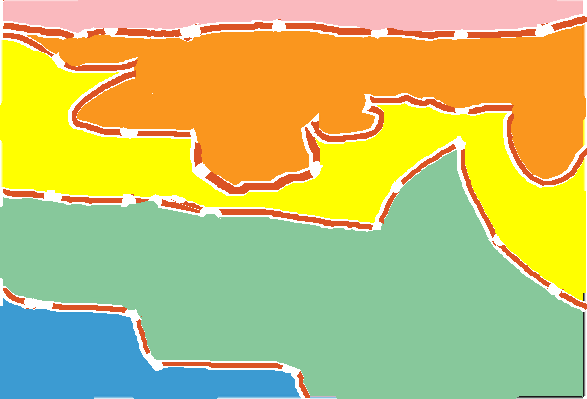
\includegraphics[height=1.9cm]{g.png}}
       \hspace*{\fill}%
    \label{fig:smoothTerm}%
  \end{figure}
\end{block}
	\end{footnotesize}
}

\subsection{System Configuration}
\frame{\frametitle{The Metric Labeling Problem}%\framesubtitle{\insertsubsection}
  \framesubtitle{System Configuration}

\begin{table}[b]
  \caption{Design choices summary}
  \label{tab:method}
  % \begin{tabular}{>{\centering\bfseries}m{1in} l}
  \begin{tabular}{cl} \hline
		$\mathcal{S}$ & {\footnotesize Quick-Shift super-pixels} \\
								&{\footnotesize  Background Echotexture: encoded in Appearance and SIFT-BoW}\\
		$D(\cdot)$ & {\footnotesize Echo Pattern: encoded in Appearance, Atlas and Brightness}\\% \tikz[inner sep=0mm, outer sep=0mm]{\node[inner sep=0mm, outer sep=0mm, anchor=south west] {\includegraphics[height=40pt]{featAll}};} \\
						 & {\footnotesize Acoustic Posterior: encoded in Atlas and Brightness}\\
	$V(\cdot,\cdot)$ & {\footnotesize Homogeneity }\\
		$\arg \min U(\cdot)$ & {\footnotesize Graph-Cuts} \\ \hline
  \end{tabular}
  % % \begin{tabular}{lll}
  % %  $\mathcal{S}$: Quick-Shift super-pixels &\quad &$D(\cdot)$: \\
  % %  $\arg \min:$ Graph-Cuts&&\quad Features \tikz[remember picture]{\coordinate[remember picture] (featCoord) at (0,0);}\\
  % %  $V(\cdot,\cdot)$: homogeneity as Eq.\,\eqref{eq:smoothing}& & \quad Construction { \acs{svm}-\acs{rbf}} \\
  % % \end{tabular}
\end{table}
}



 \section{Discussions}

\begin{frame}
  \begin{beamercolorbox}[wd=\paperwidth,ht=\paperheight]{frametitle}
    \begin{tikzpicture}
      \fill[nicewhite, opacity=1] (0, 0) rectangle(1, 1);
      \node [anchor=center] (cloud) at 
        (0.5\paperwidth, 0.5\paperheight)
        {\includegraphics[width=.95\paperwidth]{./images/word_cloud/results.png}};
    \end{tikzpicture}
  \end{beamercolorbox}
\end{frame}
\graphicspath{{chapters/method/figures/}}

\subsection{dummy_subsection_a}

\begin{frame}
  \frametitle{Qualitative results}
  \framesubtitle{Super-pixel classification vs Area-Overlap}
  \begin{figure}[Htbp]
    \centering
    \hspace*{\fill}%
      \subfigure[][Original Image, Ground Truth and Super-Pixels delineation.]{%
      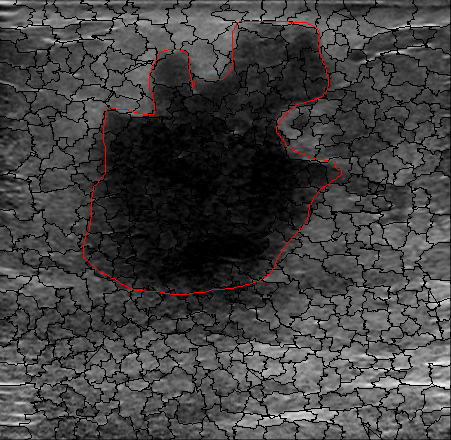
\includegraphics[width=.45\textwidth]{qualitativeResults/goodQSorigin}}
      \label{fig:dataTermb}%
      \hfill%
      \subfigure[][$\{\text{lesion}, \overline{\text{lesion}}\}$ labeling results, GT and SP delineation.]{%
      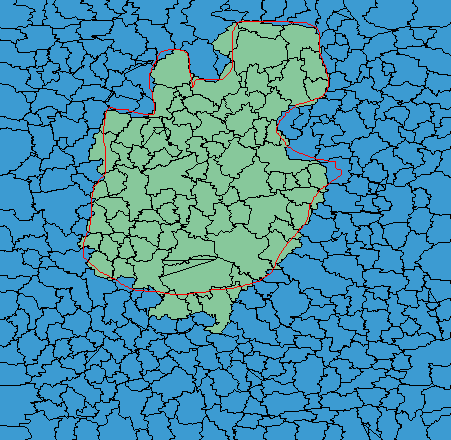
\includegraphics[width=.45\textwidth]{qualitativeResults/goodQSseg}}

      \label{fig:dataTermc}%
      \hspace*{\fill}%
        \label{fig:dataTerm}%
  \end{figure}
\end{frame}

\begin{frame}\frametitle{Qualitative results}
\framesubtitle{\footnotesize Influence of the Smoothing Term to False Positive Ratio}
\vspace{-10pt}
\begin{figure}[Htbp]
\setlength{\abovecaptionskip}{2pt}
\centering
\begin{tikzpicture}%[node distance=2cm]
  %       \node (a) {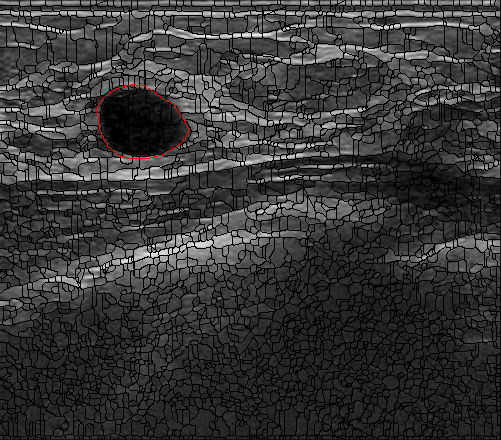
\includegraphics[width=.45\textwidth]{qualitativeResults/fporigin}};
  %%       \node [block, below of=a] (b) {B};
  %       \node [anchor=south west] (c) at ({.5\textwidth},0) {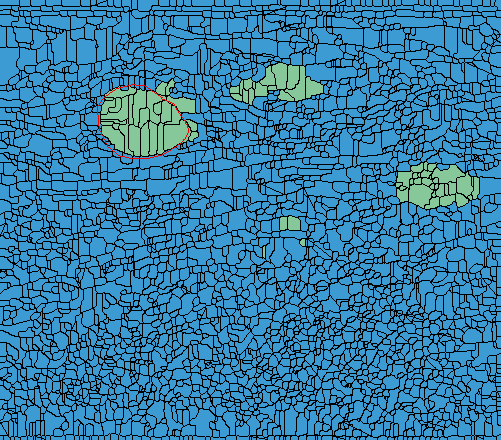
\includegraphics[width=.2\textwidth]{qualitativeResults/fpHom}};
  %       \node [anchor=north east] (d) at (a.north -| c.east) {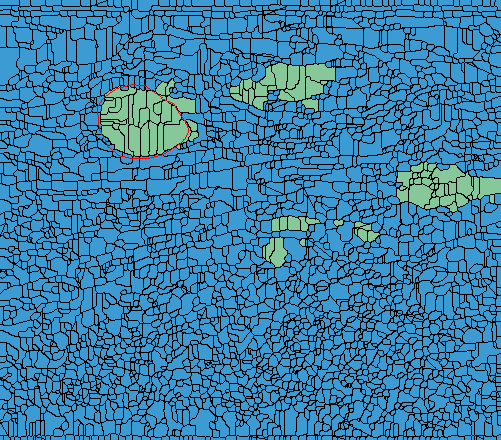
\includegraphics[width=.2\textwidth]{qualitativeResults/fpnohom}};
  %       
  \node [anchor=south west] (a) {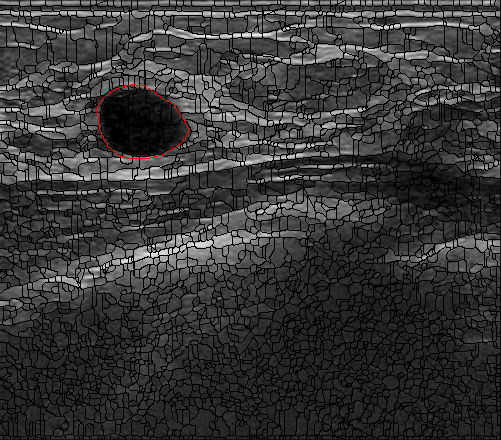
\includegraphics[height=.67\textheight]{qualitativeResults/fporigin}};
  \node [anchor =south west] (c) at ({.682\textwidth},0) {\includegraphics[height=.33\textheight]{qualitativeResults/fpHom}};
  \node [anchor = north west] (d) at (a.north -| c.west) {\includegraphics[height=.33\textheight]{qualitativeResults/fpnohom}};
\end{tikzpicture}

\end{figure}
\end{frame}

\subsection{dummy_subsection_b}
\begin{frame}[plain]\frametitle{Qualitative results}
\framesubtitle{When False Negative Emerge}
\vspace{-5pt}
\begin{figure}[Htbp]
\setlength{\abovecaptionskip}{2pt}
\centering
\includegraphics[width=.32\textwidth]{qualitativeResults/FNGT}~ 
\includegraphics[width=.32\textwidth]{qualitativeResults/FNsp}\\ \vspace{3pt}
\includegraphics[width=.32\textwidth]{qualitativeResults/FNdetected}~ 
\includegraphics[width=.32\textwidth]{qualitativeResults/FNmiss}
\end{figure}
\end{frame}


\begin{frame}[plain]\frametitle{Quantitative Results}
\includegraphics[trim=100 340 100 250,clip, height=.7\textheight]{quant.pdf} 
\end{frame}


\end{document}
